\section*{Fitting a Linear Model}

Use \myDesmos to find a \myEmph{linear} regression model. 
To do this, use the \myDesmos commands in the table above. 

\myProblemsWithContent
{
    Find the model parameters listed below.
    \begin{center}
        \renewcommand{\arraystretch}{1.4}
        \begin{tabular}{r|l|c}
            model & best fit parameters & $r^2$ or $R^2$ \\ 
            \midrule
            {\itshape Linear} 
                & $\bm{a_1} =$ \underline{\hspace{0.5in}} & $r^2 =$ \underline{\hspace{0.5in}} \\
                & $\bm{b_1} =$ \underline{\hspace{0.5in}} & \\
        \end{tabular}
        \end{center}
}
{  
    When $r^2$ is close to zero, it's not a good fit. 
    When $r^2$ is close to one, it is a good fit.
    Based on this, does this line seem to be a good fit?
    Explain your thinking \myEmph{as a full sentence}.
}[\small]

\myProblemsWithContent
{
    Sketch a scatterplot of the $(x,y)$ data. 
    Then sketch the line $y = \bm{a_1} + \bm{b_1}x$ based on \myDesmos.\newline
        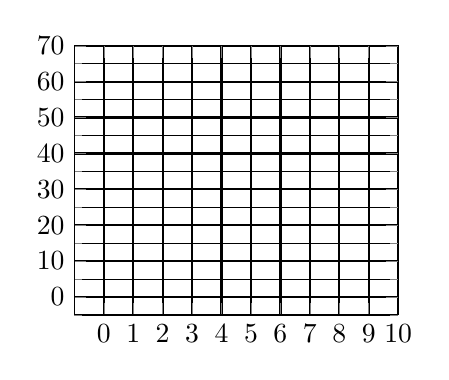
\begin{tikzpicture}
            \begin{axis}[
                scale=0.6,
                grid = both,
                xmin=-1, xmax=10, xtick distance=1, xtickmin=0,
                ymin=-5, ymax=70, ytick distance=10, minor y tick num=1,
                major grid style={solid,thick,black},
                minor grid style={solid,very thin,black},
            ]
            \end{axis}
        \end{tikzpicture}
}
{
    How many points does the line go through?
}[\small]